\documentclass{article}
\usepackage[utf8]{inputenc}
\usepackage{geometry}
\usepackage{datetime2}
\usepackage{xparse}
\usepackage{amsmath}
\usepackage{booktabs}
\usepackage{array}
\usepackage{hyperref}


 \geometry{
 a4paper,
 total={170mm,257mm},
 left=20mm,
 top=20mm,
 }

 
 \usepackage{graphicx}
 \usepackage{titling}

 \title{Assignment 1: Paper Review "Review of Artificial Intelligence Applications in Engineering"
}
% \author{Muhammad Qomaruz Zaman}
\date{18 March 2025}
 
 \usepackage{fancyhdr}
\fancypagestyle{plain}{%  the preset of fancyhdr 
    \fancyhf{} % clear all header and footer fields
    \fancyfoot[R]{}
    \fancyfoot[L]{}
    \fancyhead[L]{
\includegraphics[width=2cm]{ITS_pojok.pdf}}
    \fancyhead[R]{ \DTMnow}
}
\makeatletter
\def\@maketitle{%
  \newpage
  \null
  \vskip 1em%
  \begin{center}%
  \let \footnote \thanks
    {\LARGE \@title \par}%
    \vskip 1em%
    %{\large \@date}%
  \end{center}%
  \par
  \vskip 1em}
\makeatother

\usepackage{lipsum}  
% \usepackage{cmbright} % Change the font by zee

\begin{document}

\maketitle


\noindent\begin{tabular}{@{}ll}
    Author(s): & Azhar Basis Panrita\\
     Teacher: &  Muhammad Qomaruz Zaman, S.T., M.T., Ph.D.\\
     Class name: & Kecerdasan Buatan\\
     YouTube video link: & \url{https://-} \\
     GitHub link: & \url{https://-}
\end{tabular}
\vspace{2cm}

%Tulisan ini bisa di ganti: robotika.
%Tulisan ini juga: \lipsum[2]

\section*{1. Pendahuluan}
Paper Review "Review of artificial intelligence applications in engineering merupakan sebuah review paper yang menyoroti kemajuan terkini dan tren riset masa depan dalam penerapan AI pada konsep desain/rekayasa, mencakup 15 tahun terakhir sebagai periode percepatan AI. Metode seperti machine learning, algoritma genetika, dan fuzzy logic ditelaah secara mendalam dari perspektif desain rekayasa. Studi desain berbasis AI dikategorikan dan ditinjau secara kritis untuk berbagai tahap desain: inspirasi, ide dan konseptualisasi, evaluasi, optimisasi, pengambilan keputusan, serta pemodelan. Hasil dari review paper tersebut bertujuan agar memberikan perspektif garis besar tentang pemilihan metode AI yang sesuai berdasarkan hasil literatur untuk masalah desain \cite{yuksel2023}.

Proses desain produk dan rekayasa tradisional yang berpusat pada manusia kini mengalami transformasi besar dengan hadirnya kecerdasan buatan (AI). AI, yang didefinisikan sebagai algoritma komputer yang meniru proses mental biologis \cite{ertel2017} \cite{liu2018}, mampu melakukan pembelajaran, pemahaman, estimasi, pemecahan masalah, hingga pengambilan keputusan \cite{huang2019}. Dalam konteks desain, AI mendukung operasi kompleks seperti evaluasi, perbandingan, dan optimisasi, sehingga desainer dapat lebih fokus pada aspek kreatif dan inovatif. Keunggulan AI dibanding manusia terletak pada kemampuan komputasi tinggi, pemrosesan big data, serta pengambilan keputusan yang objektif \cite{liao2020} \cite{allison2022}.

Metode klasik seperti fuzzy logic, algoritma genetika, expert systems, dan artificial neural networks telah lama digunakan dalam evaluasi dan optimisasi desain \cite{lu2012}. Namun, dalam beberapa tahun terakhir, metode modern berbasis data seperti machine learning dan deep learning semakin mendominasi \cite{chang2018} \cite{nasiri2021}. Berbagai penelitian menunjukkan penerapan AI di banyak bidang: desain sel fotovoltaik \cite{youssef2017}, deteksi cacat komponen mekanis \cite{chang2018}, optimisasi manufaktur aditif \cite{nasiri2021}, industri busana \cite{giri2019}, arsitektur dan rekayasa sipil \cite{lu2012} \cite{pan2021}, hingga rekayasa struktural \cite{salehi2018}. Tren masa depan juga menyoroti integrasi AI dengan teknologi lain seperti robotika, VR/AR, blockchain, dan printer 4D \cite{pan2021}.

Kontribusi utama kajian ini dapat dirangkum sebagai berikut:
\begin{itemize}
    \item Menyajikan tinjauan komprehensif aplikasi AI dalam desain produk dan rekayasa selama 15 tahun terakhir \cite{saridakis2008} \cite{verganti2020}.
    \item Menentukan ruang lingkup dan batasan praktik saat ini.
    \item Memberikan panduan bagi desainer dalam memilih metode AI yang sesuai dengan masalah desain.
    \item Memproyeksikan arah penelitian AI di bidang desain ke depan.
\end{itemize}

Secara keseluruhan, penelitian ini menekankan pentingnya menggabungkan metode klasik (rule-based) dan modern (data-driven) dalam satu kerangka komprehensif. Dengan cara ini, desainer dapat menemukan solusi AI yang lebih efisien, akurat, dan menyeluruh untuk berbagai tahap desain mulai dari ideasi, konseptualisasi, evaluasi, optimisasi, hingga pemodelan.

\section*{2. Metodologi}
Penulis menggunakan pendekatan systematic literature review (SLR) dengan rentang waktu 2006–2021. Artikel yang relevan diklasifikasikan berdasarkan:
\begin{figure}[tb]
    \centering
    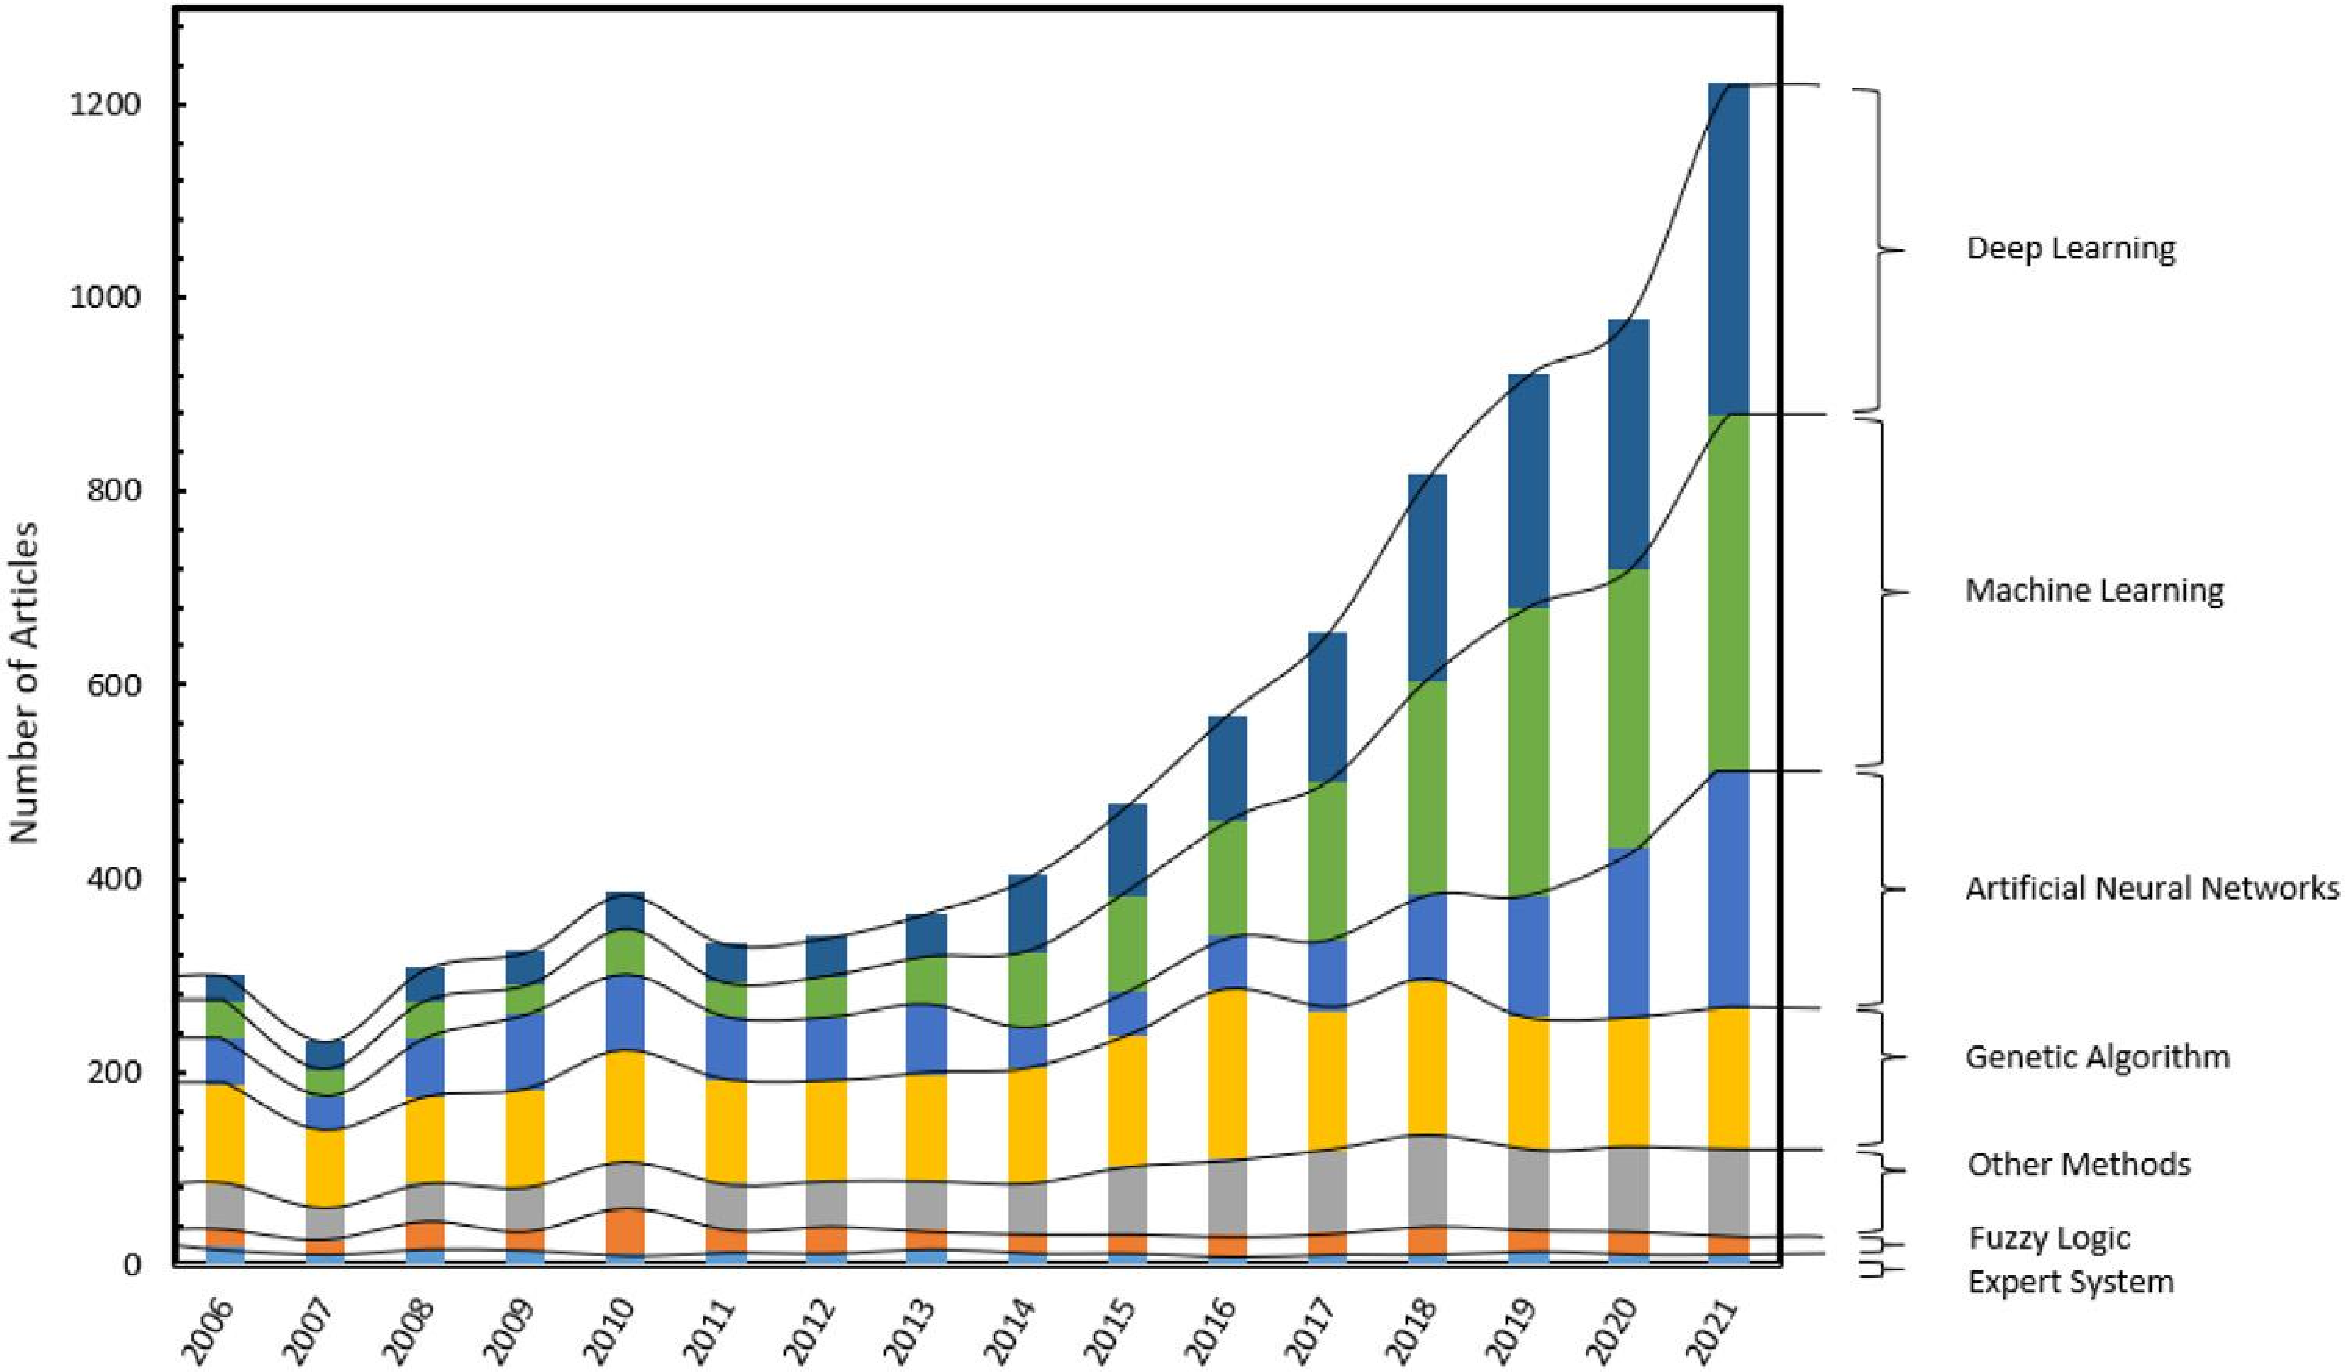
\includegraphics[width=0.7\linewidth]{ArticalAIPublished.pdf}
    \caption{Number of articles published per year}
    \label{fig:enter-label}
\end{figure}

\begin{itemize}
    \item \textbf{Jenis metode AI} (klasik vs modern).
    \item \textbf{Tahapan desain rekayasa} (ideasi, konseptualisasi, evaluasi, optimisasi, pengambilan keputusan, pemodelan).
    \item \textbf{Bidang aplikasi} (mekanikal, sipil, arsitektur, manufaktur, dll.).
\end{itemize} 
Metodologi ini memastikan bahwa hasil review tidak hanya deskriptif, tetapi juga analitis dalam menghubungkan metode dengan konteks aplikasinya.

\section*{3. Konstribusi Utama}
\subsection*{a. Klasifikasi Metode AI}
\begin{itemize}
    \item \textbf{Klasik}: expert systems, fuzzy logic, artificial neural networks, genetic algorithms
    \item \textbf{Modern}: machine learning, deep learning, swarm intelligence, hybrid approaches.
\end{itemize}
\subsection*{b. Tahapan desain yang didukung AI}
\begin{itemize}
    \item Inspirasi dan ide awal.
    \item Pengembangan konsep.
    \item Evaluasi dan optimisasi.
    \item Pengambilan keputusan berbasis data.
    \item Pemodelan dan simulasi.
\end{itemize}
\subsection*{c. Tren Penelitian}
\begin{itemize}
    \item Pergeseran dari pendekatan rule-based ke data-driven 
    \item Meningkatnya perhatian pada Explainable AI (XAI) untuk meningkatkan transparansi dan kepercayaan.
    \item Meningkatnya perhatian pada Explainable AI (XAI) untuk transparansi dan kepercayaan
    \item Potensi integrasi AI dengan teknologi frontier seperti VR/AR, blockchain, dan 4D printing
\end{itemize}

\section*{4. Kekuatan Paper}
\begin{itemize}
    \item \textbf{Komprehensif}: Menggabungkan metode klasik dan modern dalam satu kerangka review.
    \item \textbf{Sistematis}: Menggunakan metodologi pencarian literatur yang jelas dan terukur.
    \item \textbf{Praktis}: Memberikan panduan pemilihan metode AI sesuai tahap desain.
    \item \textbf{Visioner}: Menunjukkan arah penelitian masa depan yang relevan dengan perkembangan teknologi industri.
\end{itemize}

\section*{5. Keterbatasan}
\begin{itemize}
    \item \textbf{Studi kasus terbatas}: Contoh aplikasi disebutkan, tetapi tidak dibahas secara mendalam.
    \item \textbf{Rentang waktu literatur}: Fokus pada 2006–2021, sehingga perkembangan terbaru (misalnya generative AI pasca-2022) belum tercakup.
    \item \textbf{Kurang empiris}: Diskusi implementasi nyata di industri masih bersifat umum, belum banyak data kuantitatif.
\end{itemize}

\section*{6. Kesimpulan}
Secara keseluruhan, paper ini berhasil menyajikan gambaran menyeluruh tentang penerapan AI dalam desain rekayasa. Kekuatan utamanya terletak pada klasifikasi metode dan identifikasi tren penelitian. Namun, keterbatasan dalam studi kasus dan literatur terbaru perlu diperhatikan bagi pembaca yang ingin menggunakan paper ini sebagai landasan penelitian lanjutan. Dengan demikian, paper ini lebih tepat diposisikan sebagai survey komprehensif daripada analisis mendalam, tetapi tetap memiliki nilai akademik tinggi sebagai peta awal bagi penelitian di bidang AI dan desain rekayasa.

% \lipsum[1][1]

% \subsection*{Heading lvl 3: Subsection: Untuk membuat bibliografi, silahkan edit file references.bib}


% Ini contoh untuk membuat bullets: \lipsum[1][2]
% \begin{itemize}
%     \item Item 1: \lipsum[1][3]
%     \item Item 2: \lipsum[1][4]
% \end{itemize}

% \lipsum[2][2]
% Kemudian ini contoh membuat numberings \begin{enumerate}
%     \item Ini contoh membuat link ke figure Citing Fig. \ref{fig:enter-label}
%\begin{enumerate}
%     \item \cite{yuksel2023}
%\end{enumerate}
%     \item Ini contoh membuat link ke 2 sitasi: Citing Refs. \cite{chen2022wireless} and \cite{jones2018wireless}
%     \item Ini contoh membuat link ke 3 sitasi: Citing Refs. \cite{chen2022wireless, jones2018wireless, lee2021machine, smith2020energy}
%     \item Ini contoh membuat link ke suatu persamaan: Citing Eq. \ref{eq:panjang dan lengkap}
%     \item Ini contoh membuat link ke suatu tabel: Citing Table \ref{tab:dummy_table}

% Dummy equation as an example:
% \begin{equation}
% \label{eq:panjang dan lengkap}
% \begin{aligned}
% \hat{y}_i &= \frac{1}{\sqrt{2\pi\sigma_i^2}} \sum_{j=1}^{N} \omega_{ij} \int_{-\infty}^{\infty} e^{-\frac{(x_j - \mu_i)^2}{2\sigma_i^2}} \nabla \cdot \left( \vec{F}_j \times \vec{A}_i \right) \, dx_j \\
% &+ \sum_{k=0}^{\infty} \frac{(-1)^k}{k!} \left( \frac{\partial}{\partial t} \right)^k \left[ \begin{pmatrix} a_{11} & a_{12} \\ a_{21} & a_{22} \end{pmatrix} \begin{pmatrix} b_1 \\ b_2 \end{pmatrix} \right]_i \\
% &+ \lim_{n \to \infty} \sum_{m=1}^{n} \frac{1}{m^2} \left[ \frac{\Gamma(z_i)}{\zeta(s_i)} \right]^{\alpha_i} \prod_{l=1}^{M} \left( \frac{c_l}{d_l} \right)^{\beta_i} \\
% &+ \begin{cases}
%     \tilde{x}_i^2 + \dot{x}_i, & \text{if } x_i > 0 \\
%     \ddot{x}_i - \bar{x}_i, & \text{otherwise}
%   \end{cases} \\
% &+ \int_0^1 \left( \frac{\partial^2 u}{\partial x^2} + \frac{\partial^2 u}{\partial y^2} \right) \breve{u} \, dx \, dy \\
% &+ \sqrt[3]{\sum_{q=1}^{Q} \left( \frac{p_q}{\tilde{p}_q} \right)^{\gamma_i}} \bigoplus \left( \frac{\partial \hat{f}}{\partial \check{x}} \right)_i
% \end{aligned}
% \end{equation}


% \begin{figure}[tb]
%     \centering
%     
\includegraphics[width=0.5\linewidth]{ITS_pojok.pdf}
%     \caption{Caption 1: Don't forget to include caption for each figure.}
%     \label{fig:enter-label}
% \end{figure}

% \begin{table}[htbp]
% \centering
% \caption{Dummy Table with Custom Formatting and Caption}
% \begin{tabular}{lll}
% \hline
% \textbf{No} & \textbf{Nama} & \textbf{Asal} \\ \hline
% 1           & Ruqoyah       & Palembang     \\
% 2           & Juminten      & Gresik        \\
% 3           & Budi          & Nganjuk       \\ \hline
% \end{tabular}
% \label{tab:dummy_table} % Add a label for referencing
% \end{table}

\bibliographystyle{IEEEtran}
\bibliography{references}



\end{document}
